\documentclass[a4paper]{article}
\usepackage{Style/DaVinci2019}
\usepackage{enumitem} % http://ctan.org/pkg/enumitem
\usepackage[none]{hyphenat}
\usepackage{hyperref}
\usepackage{pdfpages}

% The alphabetic order of the definitions is not automatic, if you change this, change that as well!
\newcommand{\Abr}{Administrative Regulations} % Bestuursregelement
\newcommand{\Asta}{Bylaws} % Statuten
\newcommand{\Ahr}{House Rules} % Huishoudelijk Regelement
\newcommand{\Asr}{Safety Rules} % Veiligheidsregelement
\newcommand{\Awr}{Contest Rules} % Wedstrijdregelement
\newcommand{\Ajv}{Annual Report} % Jaarverslag
\newcommand{\App}{Privacy Policy}
\newenvironment{g}{\color{grey}}{}
\newenvironment{defi}{\color{accent2}\bfseries}{}

\setTitle{House Rules}
\setSubtitle{April 2019 - {\color{accent2}Proposal for GA 33}}
\enableFooter
\linenumbers
\setFooter{Huishoudelijk Regelement}

\begin{document}
\newpage
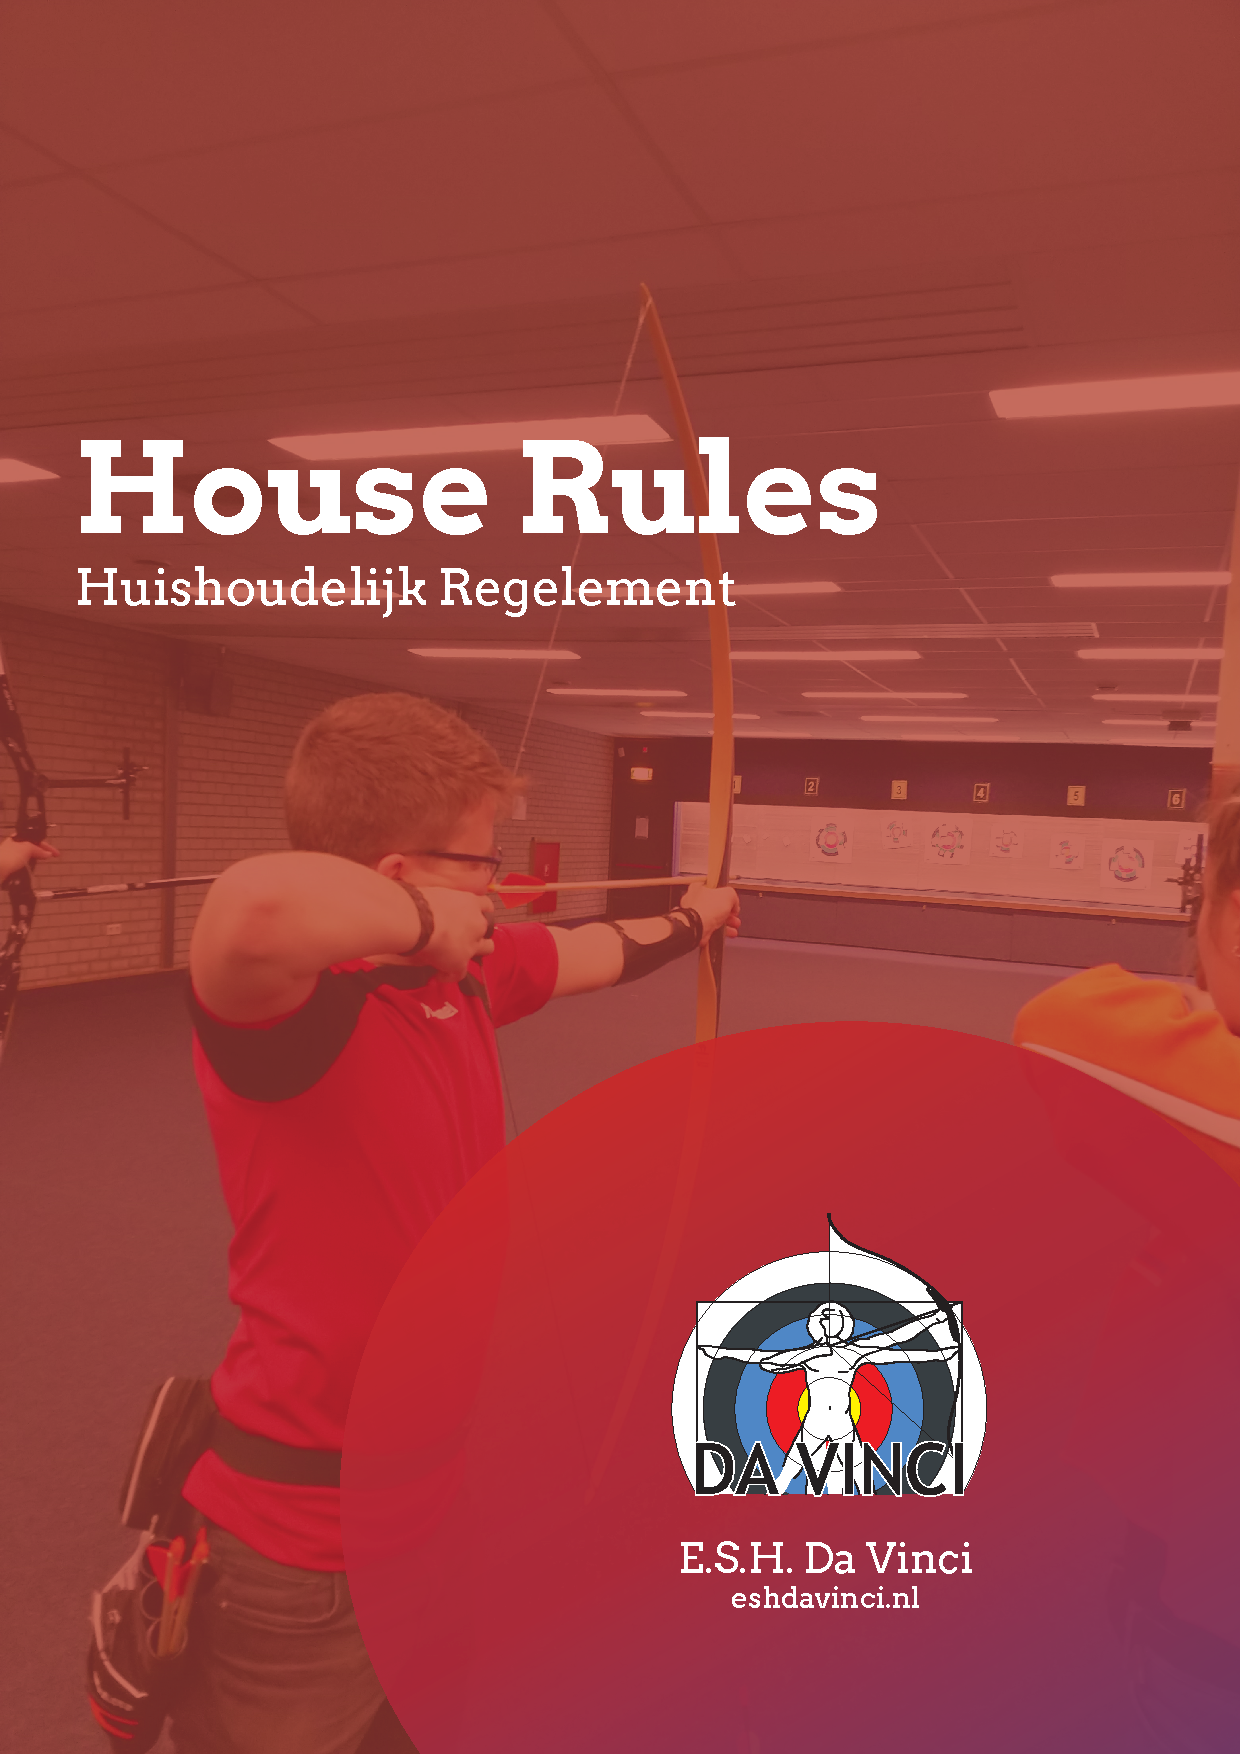
\includepdf[fitpaper=true, pages=-]{Cover.pdf}
\tableofcontents
\pagebreak
\section*{List of Definitions}
{\g Definitions can be recognized by their color and bold print throughout this document. Board Member roles are spelled with a capital (Chairman, Secretary, Treasurer)}

\bigskip

\begin{description}[font=\sffamily\bfseries, leftmargin=1cm, style=nextline]
\item[{\defi Accommodation}] Our accommodation ("Aan de Meet") consisting of the Shooting Range, Outdoor Range and the {\defi Club Room}.
    \item[{\defi ADM}]
    Aan de Meet, the association in charge of the maintenance and renting of our {\defi Accommodation}.
\item[{\defi \Abr}] Document detailing the actions that the board needs to take during the year.
\item[{\defi \Ajv}] Document detailing the actions of the board during the previous year.
\item[\defi Archer] Everyone at Da Vinci, including {\defi guests}, {\defi Members}, {\defi beginners}, {\defi Recreationists} and trainers.
    \item[{\defi Association Year}]
    Parallel to the financial year; starting September 1st and ending the 31st of August. 
\item[{\defi Beginner}]
Participants to the {\defi Beginners' Course} Beginners are required to have a valid sports card. Beginners are by definition {\defi inexperienced} archers.
\item[{\defi Beginners' Course}] Course given to beginners during the year.
    \item[{\defi “Behind the line”}]
    The side of the Shooting Line where the targets are NOT placed. 
  \item[{\defi BM}]
    Board Meeting (BV)
\item[{\defi \Asta}] Articles of Association for Da Vinci ("Statuten")
\item[\defi Club Materials] Club Materials include bows, arrows, personal protection material, spare parts, (outdoor) targets, target faces, other material owned by the club and are used for archery.
\item[{\defi Club Room}] Also known as “het hok”. It is the lockable area/room behind the shooting range, assigned for use by E.S.H. Da Vinci.
\item[{\defi \Awr}] Document stating regulations for Contests and Competitions.
\item[{\defi Downrange of the Line}] The area on the side the {\defi shooting line} where the targets are located. Opposite of {\defi ``behind the line''}.
    \item[{\defi ESSF}]
    Eindhovense Studenten Sport Federatie (Eindhoven Student Sport Federation)
\item[{\defi Experienced - Inexperienced}] The Board determines if {\defi archers} are experienced, or inexperienced depending on their safety level and skills.
\item[{\defi External Member}]
{\defi Archers} that are members of the E.S.H. Da Vinci association, but are {\defi NHB} member through another club.
  \item[{\defi GA}]
    General Assembly or General Members Meeting (ALV)
\item[{\defi General Training}] Training given by the trainers during a defined time.
\item[{\defi Guest}] Guests are people who are not associated with Da Vinci, but are invited to be present at the range. This includes spectators and archers shooting in workshops.
\item[{\defi Honorary Member}] Special title given to an {\defi archer} by the {\defi GA} for exceptional services to Da Vinci.
    \item[{\defi HR}] \Ahr\ (this document)
\item[{\defi Member}]
{\defi Archers} that are members of the E.S.H. Da Vinci association. Members are required to have a sport card from the {\defi SSC}.
    \item[{\defi NHB}]
    Nederlandse Handboog Bond (Dutch Archery Federation)
\item[{\defi Recreationist}]
{\defi Archers} that are allowed to take part in trainings. Recreationists are required to have a sport card from the {\defi SSC}.
    \item[{\defi \Asr}]
    The Safety Regulations of E.S.H. Da Vinci can be found in this {\defi HR} under Chapter 1.
    \item[{\defi Shooting Line}]
    The line, marked on the floor, from where the {\defi archer} shoots his arrows towards the target.
    \item[{\defi SSC}]
    Student Sports Centre Eindhoven (also SSCE)
\item[{\defi Supervisor}] Someone instructing {\defi archers}, ensuring safety. Supervisors are: Board Members, official trainers, competition leader(s), and those appointed by the board.
    \item[{\defi TU/e}]
    Technische Universiteit Eindhoven (Eindhoven University of Technology)
    \item[{\defi Waiting Line}]
The line placed behind, and parallel to, the {\defi shooting line}. Only {\defi supervisors}, trainers and {\defi archers} currently shooting their turn are allowed to be in the space between the {\defi shooting line} and the {\defi waiting line}. 
  \item[{\defi Workshop}]
    An event organized for an external party, with an aim of presenting the sport to outsiders. If desired it is possible to try out archery under guidance of experienced {\defi archers}.
\end{description}

\pagebreak

\section{Safety Rules}
\label{safety}
The Shooting Range is a safe place, provided that safety rules described here are followed. Every {\defi archer} must know and observe these rules. We also expect {\defi archers} to ensure others abide by these rules. \\

{\defi Archers} violating these rules may be removed from the Shooting Range. \\

\subsection{General}

\begin{enumerate}
  \item {\defi Archers} must at all times use common sense and observe the safety of everyone.
  \item All {\defi archers} must immediately follow instructions from {\defi supervisors}. The correctness of such instructions is not open for discussion until the instructions have been complied with.
  \item {\defi Inexperienced} {\defi archers} are only allowed to shoot under supervision, and should strictly follow all instructions from their {\defi supervisors}. {\defi Experienced} {\defi archers} are allowed to shoot unsupervised.
  \item Aiming a bow at persons or animals is strictly forbidden (even without an arrow on the bow).
  \item When drawing and/or shooting the bow, the angle of the arrow with the ground (elevation) may never exceed 30$^\circ$. Shooting straight up is strictly forbidden.
  \item A drawn bow without an arrow on it may never be released. Doing so may cause the bow to shatter, causing injury and/or damage.
\end{enumerate}

\subsection{Shooting Protocol}

\begin{enumerate}
  \item Bows may only be drawn at the {\defi shooting line}, and only when aimed in the direction of the targets. This also holds when there's no arrow on the bow.
  \item Arrows may only be placed on the bow when at the {\defi shooting line}. The arrow tip must always be pointed in the general direction of the targets, or the ground.
  \item {\defi Archers} may only take place at the {\defi shooting line} when there is no person {\defi downrange of the line} {\bf and} (for the indoor range) the back door is closed. Until that time, they must wait behind the {\defi waiting line}.
  \item During shooting only active {\defi archers} and {\defi supervisors} may be at the {\defi shooting line}. Everyone else, including {\defi archers} who finished shooting, must wait behind the {\defi waiting line}.
  \item If, during shooting, anyone is found to be {\defi downrange of the line}, or (for the indoor range) the backdoor is found to be open, all {\defi archers} will immediately stop shooting. Shots are aborted, not finished, and the arrows must be removed from the bows.
  \item When all {\defi archers} have finished shooting, everyone may fetch their arrows collectively.
\end{enumerate}

\subsection{Ranges}

\begin{enumerate}
  \item There may be no objects (such as targets or scoring boards) on the floor within 3 meters of the target wall.
  \item There will be no running, jumping, pushing, etc. on the range. Reckless behavior is prohibited.
  \item Bows should be put in the designated areas, or in the bow rack.
  \item Spectators are not allowed downrange of the {\defi waiting line}, unless explicitly permitted by supervisors.
\end{enumerate}

\subsection{Outdoor Range}
\label{rules:outdoor}

\begin{enumerate}
  \item {\defi Archers} are required to wear closed shoes on the outdoor range to protect against obscured arrows stuck in the grass.
  \item {\defi Archers} who are shooting on the outdoor range must confirm that all {\defi archers} have returned after fetching their arrows, including those shooting at the 70 or 90 meter targets.
\end{enumerate}

\pagebreak

\section{General}
\subsection{Goal and Scope of the \Ahr}
These {\defi \Ahr} supplement the {\defi \Asta} with regards to rules and conditions contributing to the day-to-day functioning of the association. {\defi Members} (including the board) and {\defi Recreationists} are tasked with knowing the contents of this document and following the described rules, which will be enforced by the board.

\subsection{Incorporation of the Association}
The association is incorporated at the Kamer van Koophandel under number 17174167. The association is also a member of the {\defi ESSF}, based at the {\defi SSC}, and the {\defi NHB} under number 1364.

\subsection{Changes to the \Ahr}
Proposals to change the {\defi \Ahr} shall be submitted at least 14 days in advance of the next {\defi GA} by at least three {\defi Members}, or the board. An overview of these changes will be communicated by written notice by the board at least 7 days in advance of the {\defi GA}. Proposed changes to the {\defi \Ahr} will only go into effect after they have been approved by the {\defi GA}. Changes in the {\defi \Asr} can be implemented directly by the board, without {\defi GA} approval, as they improve safety. Changes to the {\defi \Asr} have to be discussed in the next {\defi GA}.

\subsection{Validity of the \Ahr}
The {\defi \Ahr} will be declared invalid upon dissolvement of the association, or when the {\defi \Asta} are changed. Upon changing of the {\defi \Asta} , the {\defi \Ahr} have to be re-approved to make sure that they do not contradict the {\defi \Asta}. The {\defi \Ahr} should be checked at least once a year for inconsistencies with day-to-day rules, and updated if necessary. New rules decided upon by the {\defi GA} should also be added to the {\defi \Ahr}.

\subsection{Availability of the \Ahr}
\label{section:available}
At least one printout of the {\defi \Ahr} and {\defi \Asta} should always be present at the training location. Every {\defi Member} and {\defi Recreationist} is entitled to review these regulations, to make sure that nobody can claim unfamiliarity with these rules. The {\defi \Ahr} and {\defi \Asta} should also be available on the E.S.H. Da Vinci website.

\subsection{Fines and Suspensions}
\label{rules:ban}
Whenever an {\defi archer}, thus including {\defi guests}, infringes upon one or more articles from the {\defi \Asta , \Ahr} or {\defi \Asr}, or in case of infringing upon regulations based on the rules described in these documents, the board can punish the violator with a fine and/or suspension. The severity of this measure will be determined depending on the specific infringement. In case of disagreement between the board and the offender, the matter will be mediated by a {\defi GA}.

\subsection{\App}
As the association processes personal data for {\defi guests}, {\defi (external) Members}, {\defi beginners}, {\defi Recreationists} and trainers, a document detailing the processing and storage of personal data, the \App\, needs to be available to all affected, in accordance to the \textit{Algemene verordening gegevensbescherming} (AVG), as entered into Dutch law on the 25th of May 2018.

\subsubsection{Availability}
The \App\ should always be made available together with the {\defi \Ahr}, as specified in Section \ref{section:available}. All affected, including {\defi guests}, are permitted to view this document.

\subsubsection{Changes}
The board is permitted to change the \App\ if regulations change in Dutch law, if contracted third parties require different data for daily functions and if the association requires different data for daily function of the association. Changes for other reasons, such as but not limited to gathering more data for statistical purposes, or the addition of new third parties, requires explicit {\defi GA} approval. \\

If the \App\ is changed, a written notice stating changes, and distributing the new \App\ will be sent by the board to all affected, including but not limited to {\defi Members}, {\defi Recreationists} and trainers. Affected persons have the right to object to this change by written response within two weeks (fourteen (14) days) of the original notice by the board. If no explicit {\defi GA} approval was given, explicit {\defi GA} approval will be required upon objection of an affected person.


\section{General Assembly}
\subsection{Organization}
\label{section:yearlyGA}
The board is obliged to, as stated in {\defi \Asta} Section 14.1, organize a {\defi GA} at least once every year and they may organize a {\defi GA} at any time. The board shall provide an agenda and invitation and send these together with the announcement of the date of the {\defi GA}. Any {\defi GA} is convened by written notice to all {\defi Members} and {\defi Recreationists} at least seven days prior, as specified in \Asta\ Section 15.3. At the yearly {\defi GA}, the board is obliged to report the {\defi \Ajv} and to present and explain the Realization, in accordance to the {\defi \Asta} Section 14.1. \\

As stated in {\defi \Asta} Section 15.2, the board can be required to organize a {\defi GA} within two weeks, if at least one tenth of the {\defi Members}, eligible for voting at the {\defi GA}, request them to do so. The normal procedure for {\defi GA} announcement, as detailed above, will then be followed. If the board fails to organize a {\defi GA}, the requesters will choose their own chairman for this {\defi GA}, who will send the written notice to all {\defi Members} and {\defi Recreationists}. \\

\subsection{Voting}
The voting or poll takes place as a rule by show of hands and in person, or by proxy (you can vote by proxy for only two {\defi Members}, as specified in {\defi \Asta} Section 12.2). If the board, or at least one {\defi Member} or {\defi Recreationist} deems it desirable, the chairman may decide to a written vote or poll, in accordance to {\defi \Asta} Section 12.4. If a vote or poll concerns people (for instance the choosing of a new board), it shall always be a written vote. \\ 

In the event of a written vote, the chairman designates a voting committee consisting of two members. The board provides authenticated voting papers. The numbers of voting papers handed in must be equal to the numbers of voting members present, combined with the amount of votes by proxy. The committee counts the votes and checks the validity of the votes. The committee will announce the result of the vote to the {\defi GA}. \\

A voting ballot shall be declared invalid in case of the following: it is signed, the paper is not marked by the board, the ballot is unreadable/unclear or if it contains a choice that was not part of the set of choices that is currently being voted on.

\section{Accommodation}
\subsection{Opening Hours}
\label{section:opening}
The {\defi Accomodation} is opened at the regular training times during the {\defi TU/e} academic year, except when communicated otherwise by the board. Exact dates and times are published on the website and communicated by the board in advance. Regular training times are {\g (2019)}: \\

\begin{tabular}{lll}
Monday    & 18.00-20.00 & Free Practice  and {\defi Beginners’ Course}s \\
          & 20.00-22.00 & {\defi General Training} (with a trainer)     \\
Wednesday & 18.00-20.00 & Free Practice and  {\defi Beginners’ Course}s  \\
          & 20.00-22.00 & Free Practice                        
\end{tabular}

\bigskip

If all the shooting lanes on the range are in use during a {\defi Beginners’ Course}, other {\defi Members} or {\defi Recreationists} are not allowed to shoot. The board will communicate the dates of the {\defi Beginners’ Course} to {\defi Members} and {\defi Recreationists}.

\subsubsection{Entrance}
On Wednesday evenings Da Vinci is not allowed to use the front door to enter or exit the Shooting Range, instead you can use the back door. If on any other day the front door can not be used, the board will clearly communicate this to the {\defi archers}. 

\subsection{Maintenance and Cleaning}
{\defi Members} and {\defi Recreationists} can be requested to help with maintenance and cleaning of the {\defi Accomodation} by the board. Maintenance costs will be paid for by the association.

\subsubsection{Small tasks}
{\defi Members} and {\defi Recreationists} are expected to perform small maintenance, such as throwing out the trash, themselves without board involvement.

\subsection{Shooting Range}
\subsubsection{Entrance Requirements}
The Shooting Range can be used by {\defi Members} and {\defi Recreationists}. {\defi Guests} need explicit permission from the board to use the Shooting Range. 

\subsubsection{Allowed Materials on the Shooting Range}
Only traditional, recurve and compound bows are allowed on the Shooting Range. Shooting with crossbows, firearms or other weapons is forbidden. When introducing a different kind of bow, approval from the board is required. In general, only equipment allowed by Dutch law and the {\defi NHB} regulations is allowed, except restricted further above.

\subsection{Outdoor Range}
\label{section:outdoor}
The Outdoor Range offers some flexibility around opening hours. If the gates of the {\defi Accommodation} are open, or the {\defi Member} is in possession of a gate key, {\defi Members} can use the Outdoor Range outside regular opening hours under the following conditions:

\begin{enumerate}
\item The {\defi Member} uses their own material (bow, arrows).
\item The {\defi Member} is an {\defi experienced} {\defi archer}, who is able to hit at least the 30 meter target without problems.
\item The {\defi Member} needs to be aware of the safety regulations for the Outside Range, as described in Section \ref{rules:outdoor}, and must comply to these rules. Non compliance will lead to punishment, as specified in Section \ref{rules:ban}.
\end{enumerate}

The gates are not always open: if the gates are closed it’s not possible to use the range, except as specified in Section \ref{sec:gatekey}. \\

Use of the Outdoor Range outside regular opening hours by {\defi Recreationists} is only allowed in the presence of a board member or a {\defi Member} approved by the board. In all other situations it is absolutely forbidden for a non-{\defi Members} to train on the outdoor range, outside regular training hours. 

\subsubsection{Gate Keys}
\label{sec:gatekey}
{\defi Members} can obtain a Gate Key through the board in exchange for a fee, as specified by the {\defi ADM}. After receiving a Gate Key, rules from {\defi ADM} apply regarding the ownership of the key. {\defi Members} that return the key after the end of their membership will get the fee (as it was at the time of getting the key) returned from Da Vinci. If a {\defi Member} does not return the key after the end of their membership, the rules from Section \ref{section:outdoor} still apply, and they will thus not be allowed to use Da Vinci targets.

\subsubsection{Use of Materials from the Club Room}
When using the Outdoor Range outside of Da Vinci opening hours, {\defi archers} are never permitted to enter the {\defi Accommodation}, including but not limited to the {\defi Club Room}, except with express permission from {\defi ADM}. Those wishing to shoot outside of Da Vinci opening hours are therefore responsible for bringing their own equipment with them.

\subsection{Club Room}
\subsubsection{Usage rules}
The {\defi Club Room} may be used by {\defi Members} and {\defi Recreationists} at Da Vinci, as well as by participants of the {\defi Beginners' Course}, as well as those who have been granted access by the board. 

\subsubsection{Safety}
To prevent holdups at the Shooting Range, the door {\defi downrange of the line} will be closed whenever nobody is present, or when {\defi archers} are present for longer than a minute. The door will only be reopened after knocking, in accordance with the {\defi \Asr}.

\subsubsection{Storing personal belongings}
{\defi Members} and {\defi Recreationists} are permitted to store their archery equipment, such as bows and arrows in the {\defi Club Room} in spots designated for storage, as decided by the board. These materials are stored without any insurance policy, and are stored at own risk. The board will ensure safety of stored materials on a best effort basis. Stored items must be labeled with some indication of the owners identity. The board may also request the removal of items with a one month notice.

\section{Club Materials}
\subsection{Use}
{\defi Club Materials} can be used by any person who is permitted by the board to use the materials. The board can always limit usage of {\defi club materials} if needed, for instance by allocating them to Beginners or Guests. The {\defi club materials} are primarily used during the {\defi Beginners' Course} and {\defi workshops}, other usage is permitted only if it does not hinder these activities.

\subsection{Maintenance and Repairs}
\subsubsection{Beginners' Course and Workshops}
During the {\defi Beginners' Course} and {\defi workshops}, {\defi supervisors} are responsible for inspecting the material for damage at the beginning and end of each training or {\defi workshop}. Damaged materials must not be used until repaired if safety is compromised.

\subsubsection{General}
The board is responsible for preventative and corrective maintenance of the {\defi club materials} to ensure the materials are safe to use. The board can delegate maintenance to a committee.

\subsubsection{Damages}
In case of any damage during usage in {\defi General Training}, free practice or external use, the {\defi archer} who used the bow is responsible for contacting the board. In case the damage occurred due to misuse, the {\defi archer} is also responsible for repair costs. In case of normal wear and tear it is highly appreciated that {\defi archers} who use the material play an active role in repairing it.

\subsection{Internal Use}
\subsubsection{Beginners}
{\defi Beginners} are required to use {\defi club materials} during the Beginners' Course, unless specified otherwise by the board.

\subsubsection{General}
After the {\defi Beginners' Course}, {\defi Members} and {\defi Recreationists} are allowed to use the Club Materials during training and free practice. In case there are not enough bow and/or arrows available, the bows are distributed on a first come first serve basis.

\subsection{External Use}
{\defi Members} and {\defi Recreationists} are allowed to borrow materials owned by Da Vinci and seen as {\defi club materials}, for use in external competitions, by requesting this through the board. When borrowing, a fee is required equal to 1 euro {\g (2019)} for each period between {\defi Accommodation} opening hours. If the bow is not returned before the beginning of the next time that the {\defi Accommodation} is open, a fee of 0,50 euros {\g (2019)} is required. A deposit of 50 euros additionally needs to be paid, any damage needs to payed from this deposit. In case damage exceeds the amount of the deposit, the member is still required to pay for the damage. \\

In case {\defi club material} is needed for a {\defi Beginners' Course}, the material needs to be returned in good working order, at the latest at the start of the lesson. In case the material is not in good order or returned too late, a fine of 10 euros is to be paid. If no valid reason is provided for not returning the material in good order on time, the board can decide that the member is no longer allowed to use {\defi club materials}.

\section{Members and Recreationists}
\subsection{Requirements}
All {\defi Members} and {\defi Recreationists} are required to conform to the {\defi SSC} rules for joining sports associations, including, but not limited to, the rule requiring a valid student sport card.

\subsection{Contribution}
{\defi Members} and {\defi Recreationists} have to pay the yearly contribution, within two weeks of being requested to do so. If a {\defi Member} or {\defi Recreationist} fails to do so, the board may (temporarily) suspend them from Da Vinci, as described in Section \ref{rules:ban}. \\

Where applicable, the contribution includes the {\defi NHB} fee. Da Vinci will pay the {\defi NHB} fee on behalf of the {\defi Member}. \\

{\defi Members} or {\defi Recreationists} wanting to join after the end of the second {\defi TU/e} quartile are charged a reduced fee. \\


\bigskip
\begin{tabular}{lllll}
                         & \textbf{Fee} & \textbf{Half Year} & \textbf{Honorary} & \textbf{Half Year + Honorary} \\
\textbf{Recreationist}   & €40,-        & €20,-              & -                 & -                             \\
\textbf{External Member} & €40,-        & €20,-              & -                 & -                             \\
\textbf{Member}          & €75,-        & €55,-              & €35,-             & €20,-                        
\end{tabular}

\bigskip

It is also possible to become a financial donor, as specified in the {\defi \Asta} Section 6. The minimal donation to become a financial donor is €20,-. As specified in {\defi \Asta} Section 6.3, donors have the right to attend the {\defi General Assembly}, but do not have the right to vote. They are also not allowed to join any activities or training.

\subsection{Behaviour}
{\defi Members} and {\defi Recreationists} are always obliged follow the rules of the {\defi NHB} (and World Archery) regarding the sport and competitions, both during Da Vinci hours as well as at external competitions, where these {\defi House Rules} do not specify otherwise, as specified in {\defi \Asta\ } Section 4.4. \\

{\defi Archers} are expected to behave and represent Da Vinci appropriately as long as they are in direct association of Da Vinci. This includes that {\defi archers} who participate in external competitions will show good sportsmanship, follow up the (safety) rules and regulations for that competition. While not mandatory, assistance at and supporting activities organized by the association is highly appreciated. \\

Further regulations about safe behavior on the shooting range, as well as general competition rules, are part of the {\defi \Awr} and the {\defi \Asr} (Section \ref{safety}) .

\subsection{Clothing Rules}
\label{section:clubclothing}
At {\defi NHB} competitions, the {\defi NHB} regulations for clothing should be followed. Additionally, for {\defi (non-external) members}, the pants are required to be black, and without markings. These rules also applies if one is representing Da Vinci, for instance during the intro, the {\defi  Beginners' Course} or at another competition where one is using the Da Vinci name, or present with a larger team from Da Vinci. 

\subsection{Types}
\subsubsection{Members}
{\defi Members} of Da Vinci, as defined in {\defi \Asta}. {\defi Members} are required to be {\defi NHB} member and to have a valid sports card. {\defi Members} have the right to attend {\defi GA}s and vote there.

\subsubsection{External Members}
{\defi External Members} are a type of {\defi Members}; they have the exact same rights and obligations, except that they have an {\defi NHB} membership through another club and not through Da Vinci.

\subsubsection{Recreationists}
{\defi Recreationists} are {\defi SSC} members with a valid sports card who through the {\defi SSC} are allowed to make use of Da Vinci's facilities and materials. {\defi Recreationists} are allowed to attend the {\defi Beginners' Course}, as well as trainings and activities, to be selected by the board. \\

{\defi Recreationists} are not {\defi Members}. As a courtesy they are invited to attend {\defi GA}s as guests; they are not allowed to vote there.

\subsection{Honorary Members}
A person who has shown extraordinary effort to support or improve Da Vinci can be nominated as an {\defi Honorary Member} by the board or at least 5 {\defi Members} that are eligible to vote on {\defi GA}s.
The {\defi Honorary Membership} is awarded by the {\defi GA} if there is at least a two-thirds majority vote. {\defi Honorary Membership} can only be awarded if accepted by the nominee. \\

The {\defi Honorary Membership} is for life, unless a {\defi GA} dissolves the {\defi Honorary Membership} with a two-thirds majority vote. {\defi Honorary Members} have the right to attend and speak at {\defi GA}s, but they do not receive a vote. They are also welcome to join (internal) competitions and club activities. When not registered as either a {\defi Recreationist} or {\defi Member}, {\defi Honoraries} cannot attend regular training. \\

The {\defi Honorary Membership} is a title unrelated to normal membership. However they can also be regular {\defi Members} assuming they satisfy the relevant conditions. In this case, they also pay a reduced fee.

\section{Board}
More information about the actions that the board needs to take are detailed in the \Abr .
\subsection{Communication}
The board has to hold {\defi BM}s as often as the chairman or two other board members find this necessary. \\

The board needs to communicate all information that is important for {\defi Members} and {\defi Recreationists} and the association, to all {\defi Members}, {\defi Recreationists} and trainers. All general notifications need to be communicated through the main communication method, currently the Da Vinci Info App in the Whatsapp application {\g (2019)}. Personal messages need to be emailed to the person in question, such that they can be archived. Official documents and announcements, such as {\defi GA} Agenda, Minutes, etc, need to be communicated per email. \\
 
All upcoming activities and up to date training times need to be published on the website. 
General announcements, updates about upcoming activities and urgent changes in planning will also be communicated via the main communication method, as listed above.

\subsection{Opening and Closing}
The board is responsible for opening and closing of the {\defi accommodation} on club evenings. Exceptions to regular opening times must be communicated via the website and other main methods of communication at least one week before the exception. The board is allowed to close early if:

\begin{enumerate}
\item There are no active {\defi archers} on the shooting range.
\item They have notified the early closure on a main mode of communication.
\item There are no objections within 30 minutes after notification.
\end{enumerate}



\subsection{Election}
A new board is elected during the yearly {\defi GA}, as specified in Section \ref{section:yearlyGA}, or during any other {\defi GA}, if there is no board. At least three weeks before the {\defi GA}, the board will notify all {\defi Members} and {\defi Recreationists} with a prior notification that a {\defi GA} will be held where a board will be elected. Candidates must apply for a board position by written notice to the Secretary of the current board within one week of the prior notification. The board will make the candidates known at the time the agenda for the {\defi GA} is send. Board candidates also have to submit a Policy for their board year, before the sending of the {\defi GA} agenda. Only {\defi Members} may be board candidates.

\subsubsection{Insufficient Candidates}

If there are not enough candidates to fill all required board positions, the board will notify all {\defi Members} that the application period is extended to the start of the election vote of the {\defi GA}. \\

If the candidates are not chosen to be board members by the {\defi GA}, {\defi Members} can apply for a board position during the {\defi GA}. If enough candidates are found and a board is chosen it can be installed at the same {\defi GA}. If no board is chosen, the current board will remain installed.

\subsubsection{Inability to Elect a Board}

If no new board is elected at the {\defi GA}, the effective board is entitled to suspend all activities including training, free practice and all other club activities until new candidates are found. The board is obligated to organize a {\defi GA} with the intent to elect and install a new board as soon as enough candidates have applied. \\

If no new board can be found within three months after the original {\defi GA}, the board is entitled to organize a {\defi GA} with the purpose to either elect and install a new board or, if no new board can be found, initiate the termination of the association.

\subsection{\Ajv}
The board is required to deliver a {\defi \Ajv} at the end of their board year. This {\defi \Ajv} needs to be discussed and approved at the yearly {\defi GA}. In this {\defi \Ajv} the board lists all decisions/changes made in the last year, as well as their accomplishments for the association. It should also include a vision for the future of the association.

\section{Finances}
\subsection{General}
The Treasurer is responsible for keeping track of all income and expenses in the financial administration. They are also required to submit the Budget, Balance and Realization to the {\defi GA} for approval.

\subsection{Club money box}
The club money box is the responsibility of the Treasurer and he/she must ensure that money is only used to purchase goods for the club.

\subsection{Archival}
The Treasurer is responsible for maintaining the financial administration in accordance with the applicable law. The Treasurer should furthermore make sure that all paper transactions (including declarations) are signed and properly archived. Digital transactions should also be archived digitally.

\subsection{Purchase of Goods}
The board can purchase goods for the club. Board members can spend a maximum of €50,- without consultation of the other board members, provided it is in the interests of the association. A board majority is necessary to approve a purchase of more than €50,-. In this case the purchase must be discussed and decided on during a {\defi BM}. \\

When a budget post is exceeded by €350,-, new purchases require a new budget, or approval by the {\defi GA}. All purchases that have not been announced in the budget, exceeding €350,- need to be approved through a {\defi GA}.

\subsection{Financial Committee}
The Financial Committee is appointed by the {\defi GA} to check the execution of the financial policy by the board. It checks the administration of the Treasurer to ensure correctness, traceability and adherence to the submitted budget. The Financial Committee must check the finances at least twice a year: once before the realization of the financial year, and once before the {\defi GA} halfway during the year. The Financial Committee consists of two committee members. They will be appointed during the yearly {\defi GA}. One backup committee member will also be appointed. The committee is, as specified in {\defi \Asta} Section 14.5, entitled to help by a professional, to be paid by Da Vinci, if this is necessary to verify the finances.

\section{Committees}
\subsection{Establishment}
The board can establish a committee with a clear task description by communicating its establishment at a {\defi GA} or by using a written notice, which includes the task description and the initial committee members, sent to {\defi Members} and {\defi Recreationists}.

\subsection{Dissolution}
\subsubsection{Dissolution by the board}
The committee can be dissolved by the board or {\defi GA} when they have decided that its task is accomplished or obsolete, or if all tasks have been distributed over other committees (or the board). When a committee by the board or {\defi GA} is dissolved, the board will sent a written notice of dissolution to all {\defi Members} and {\defi Recreationists}.

\subsubsection{Dissolution upon task completion}
The committee can also be dissolved automatically, if this was decided at establishment. These committees will be automatically dissolved after they have accomplished their tasks, and are used for one-time events. When such a committee has completed their tasks, a written notice of dissolution will be sent to all {\defi Members} and {\defi Recreationists} by the board.

\subsubsection{Dissolution notice}
Dissolution notices for committees should contain a date when the committee will be dissolved and a final report about their tasks.

\subsection{Structure}
Every committee has a chairman, who is responsible for presenting results to the board and maintaining order and effective task execution within the committee. Every committee will also be appointed a board member as a board contact, who will serve as a first contact point, and will stay up to date with current committee tasks.

\subsection{Reporting}
Committees are tasked with reporting their status to the board before every {\defi GA}. Committees also have to report their status to the board when asked. Committees should present regarding their committee at the {\defi GA}, provided they provide their report to the board at least 14 days before the {\defi GA}, such that the board is aware of the contents of the report.

\subsection{Committee members}
\subsubsection{Joining}
Both {\defi Members} and {\defi Recreationists} can join committees after approval of the committee chairman. The board or {\defi GA} can object to new committee members, provided that they supply both the joining member, as well as the committee itself of a written reasonable objection. The committee chairman is responsible for informing the board when members has requested to join the committee.

\subsubsection{Leaving}
Committee members can leave their committee after they have completed or transferred all their tasks. If tasks cannot be transferred to other committee members, the leaving member will have to complete their task first. The committee chairman is responsible for informing the board when members have requested to leave and can decide if one is allowed to leave the committee. \\ 

The board or {\defi GA} can also force members to leave committees, provided they supply both the leaving member, as well as the committee itself of a written reasoning.

\subsubsection{Disputes}
In case that disputes arise between the board and committees (and its members), the {\defi GA} will mediate.

\subsection{Budgets}
Committees have to pass every purchase by the Treasurer, who will approve or deny requests, except if this purchase is already approved in a budget. Purchases totaling to more than €100,- require a budget to be submitted to, and approved by the board. Budgets totaling more than €350,- have to be approved by the {\defi GA}. All committee budgets have to be communicated at a {\defi GA}.

\subsection{Workgroups}
Committees may have workgroups, which can have members from outside the committee, to take care of a very specific task. These workgroups have a chairman, who is in the committee, and reports to the committee. Budgetting, reporting, joining and leaving go through the committee. Workgroups can be established to take care of one-time tasks within the supervision of a committee, permitting members from outside the committee to help.

\section{Training and Beginners' Course}
\subsection{Beginners' Course}
\subsubsection{Frequency}
A {\defi Beginners' Course} is organized at least twice per year. A course will start at the start of every semester at the {\defi TU/e}.

\subsubsection{Duration}
The {\defi Beginners' Course} consists of 5 classes. The classes will take place during the times described in Section \ref{section:opening} and will be given in 5 consecutive weeks, if possible. In general there will be no lessons on days the {\defi TU/e} or Fontys is closed, or in exam weeks. If necessary, the board can overrule this.

\subsubsection{Fee}
{\defi Beginners} are required to pay a fee, which is determined to be 10 euros {\g (2019)}. The board can decide that a deposit needs to be paid, which will be given back to the {\defi beginner} if the {\defi beginner} attended all lessons, or if the board decides that non-attendance is justified.

\subsubsection{Rules}
{\defi Beginners} have to follow all instructions provided by the {\defi supervisors}. {\defi Beginners} need to have a valid sport card, issued by the {\defi SSC}. This sports card needs to entitle them to enroll in student sport associations.

\subsubsection{Trainers at the Beginners' Course}
The board will appoint {\defi beginners} trainers of the {\defi Beginners' Course}, trainers can be {\defi Archers} that have sufficient skills in archery.

\subsection{General Training}
\subsubsection{Frequency}
The {\defi General Training} is given once a week for two hours. The trainers and board determine the exact day and time of the training, which can be found in Section \ref{section:opening}.

\subsubsection{Rules}
To participate in the {\defi General Training}, you need to be either a {\defi Member} or {\defi Recreationist}, and follow directions from the trainers and the board. If one decides to not join the {\defi General Training}, you may shoot freely on the condition that you do not hinder the training. You should still listen to {\defi supervisors}, whether you are participating or not.

\subsection{Free Practice}
During Opening Hours (Section \ref{section:opening}) when there is no training or activity, you are allowed to shoot freely (called: Free Practice). The board may limit the free practice hours in times of expected low participation, or if activities need to be scheduled during that time. \\

To join the Free Practice you need to be either a {\defi Member} or {\defi Recreationist}, and follow directions from the board. You'll also need to be able to exercise archery without extensive supervision in a safe way ({\defi experienced} {\defi archer}). The board and trainers can decide to allow {\defi guests} to participate in the free practice.

\section{Competitions and Activities}
\subsection{General}
All internal competitions and activities are considered to be a training. Both {\defi Members} and {\defi Recreationists} can participate. Additional regulations for competitions are described in the {\defi \Awr}.

\subsection{Internal Competitions}
The board (or a assigned committee) is at least required to organize the following internal competitions: \\
\begin{enumerate}
\item \textbf{Ladder competition}: During every academic year a ladder competition is held, open to all {\defi Members} and {\defi Recreationists}.
\item \textbf{Koningsschieten}: Koningsschieten is held in the week of the founding of Da Vinci, as close as possible to the 2nd of February.
\end{enumerate}

\subsection{External Competitions}
\subsubsection{Yearly NHB competitions}
Da Vinci {\defi Members} can participate in yearly {\defi NHB} competitions (such as the bondscompetitie) both individual as well as in teams. The board is responsible to notify {\defi Members} that they can participate, the board is also responsible for subscribing {\defi Members} and teams. In case {\defi Members} participate in one of these competitions, the board will publish competition dates on the website. During the whole competition members are required to wear the club clothing, as described in Section \ref{section:clubclothing}.

\subsubsection{Other competitions}
The board should relay invitations to other competitions and publish dates.
\end{document}